

\begin{frame}[allowframebreaks]{Teaser: Digital editions -- some examples}

    \href{http://gams.uni-graz.at/o:ufbas.1563\#Eintrag-149}{GAMS ufbas}

    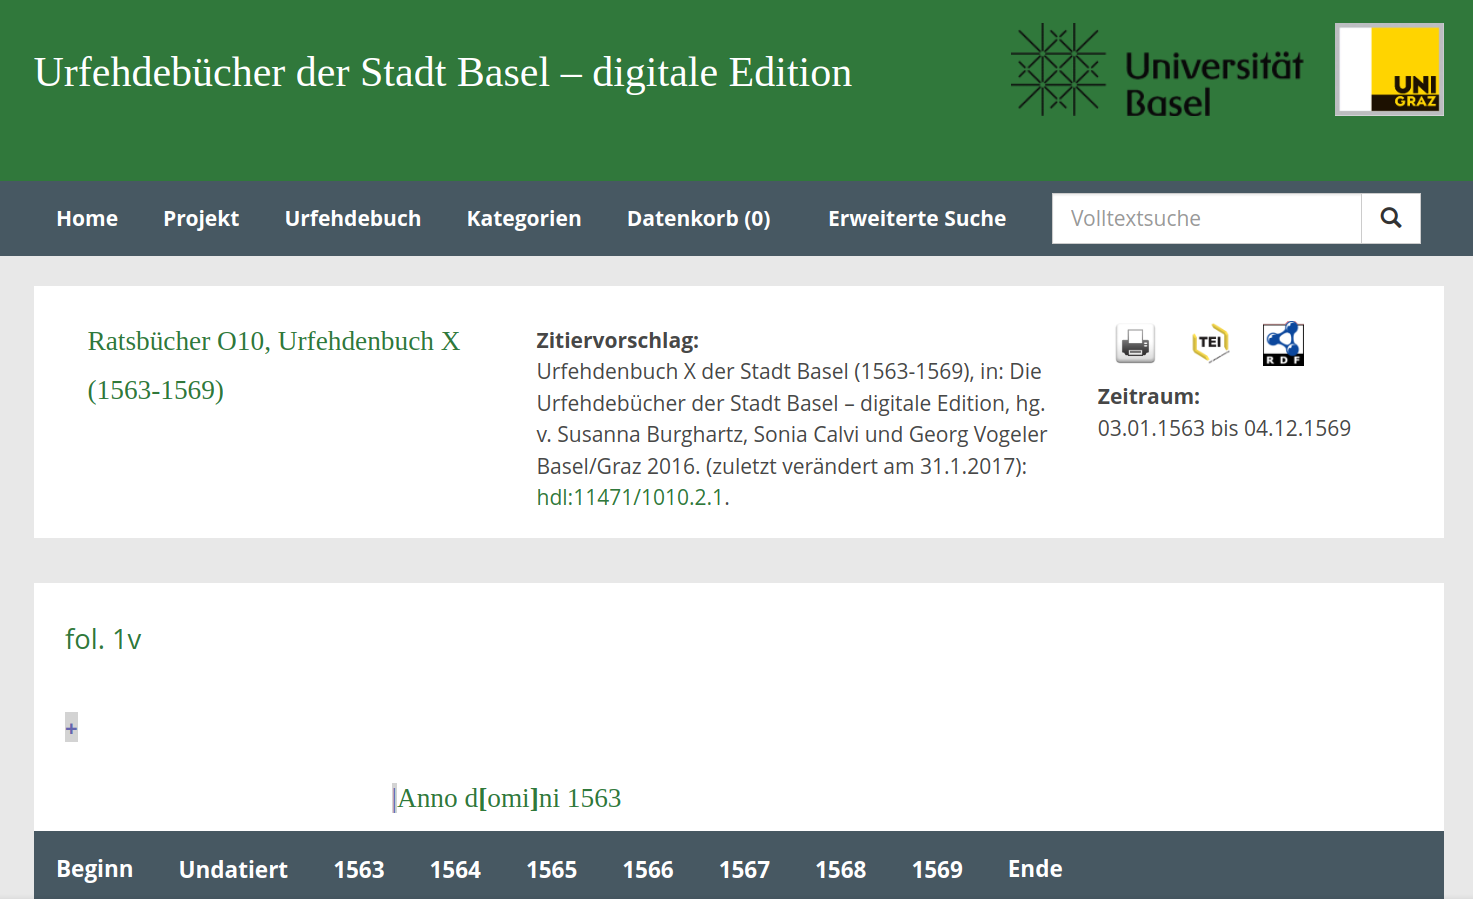
\includegraphics[width=0.48\textwidth]{img/ufbas1.png}
    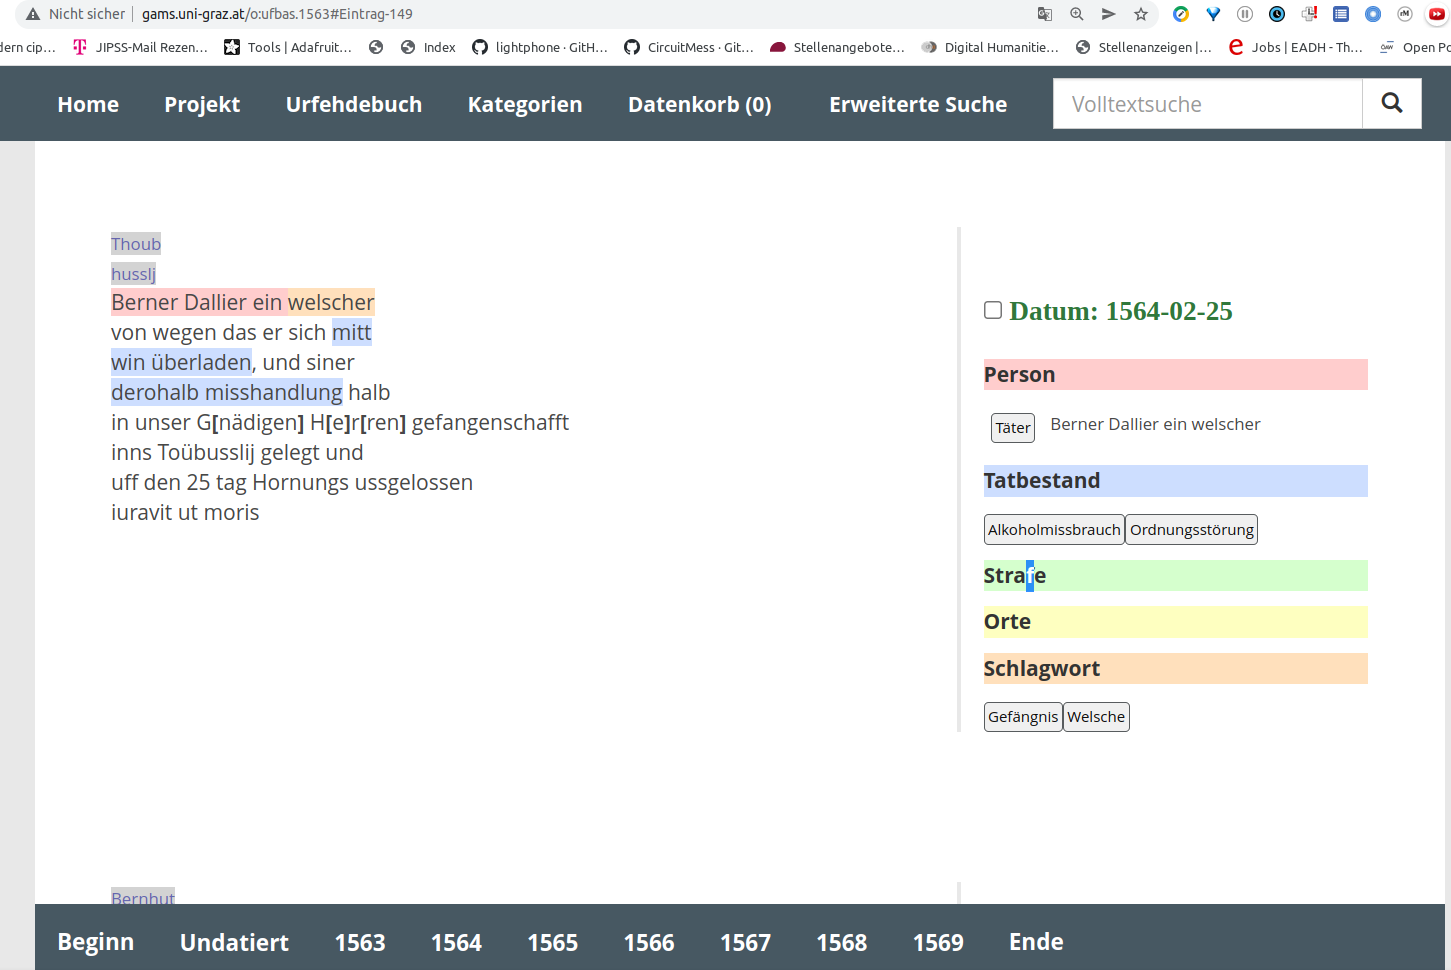
\includegraphics[width=0.48\textwidth]{img/ufbas2.png}
    
    \framebreak
    
    \href{https://gams.uni-graz.at/o:corema.pa1.recipes}{CoReMA} $\to$
    Look at: \protect\url{http://gams.uni-graz.at/corema}
    
    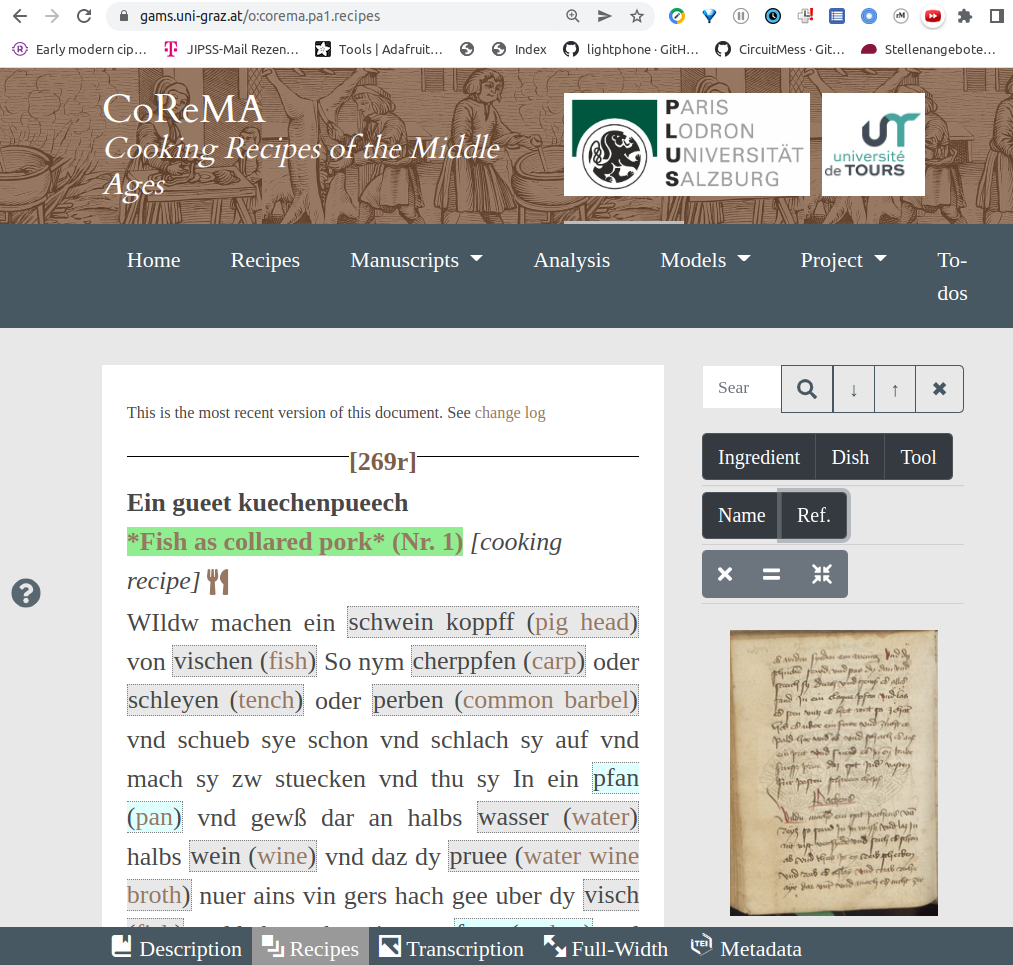
\includegraphics[width=0.6\textwidth]{img/corema-b1.png}
    
    \framebreak
    
    \href{https://furnaceandfugue.org}{Furnace and Fugue} (music in MEI, text and images)
    \begin{columns}
    \column{0.63\textwidth}
    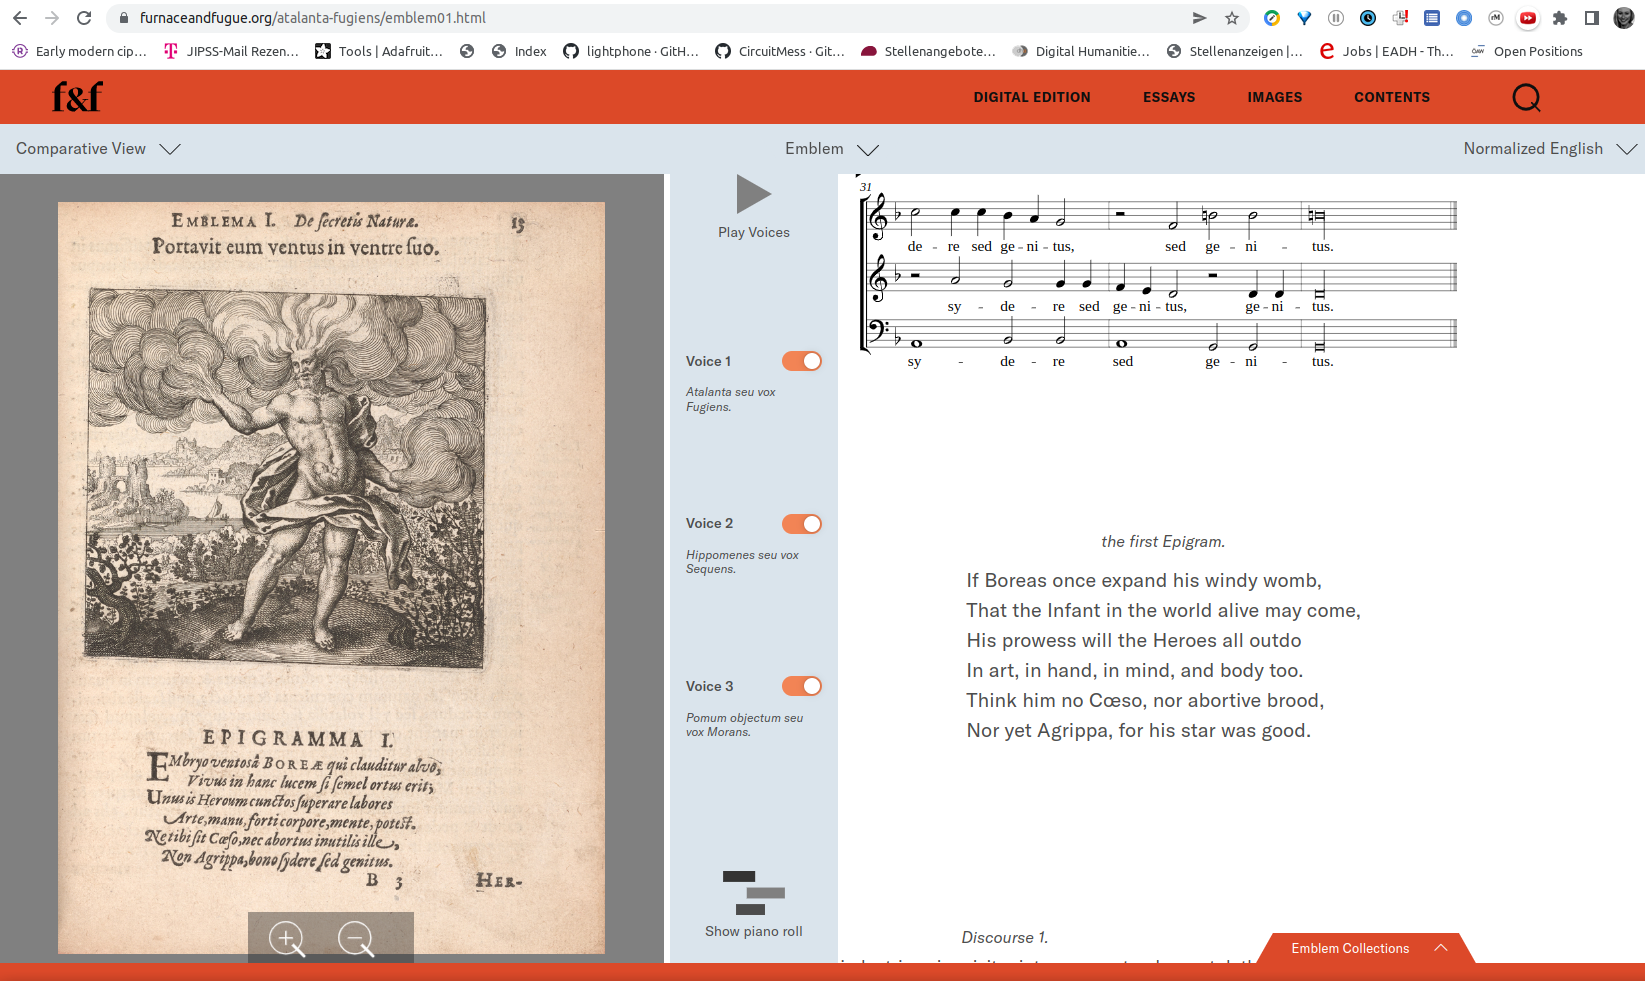
\includegraphics[width=\textwidth]{img/fnf1.png}
    \column{0.33\textwidth}
    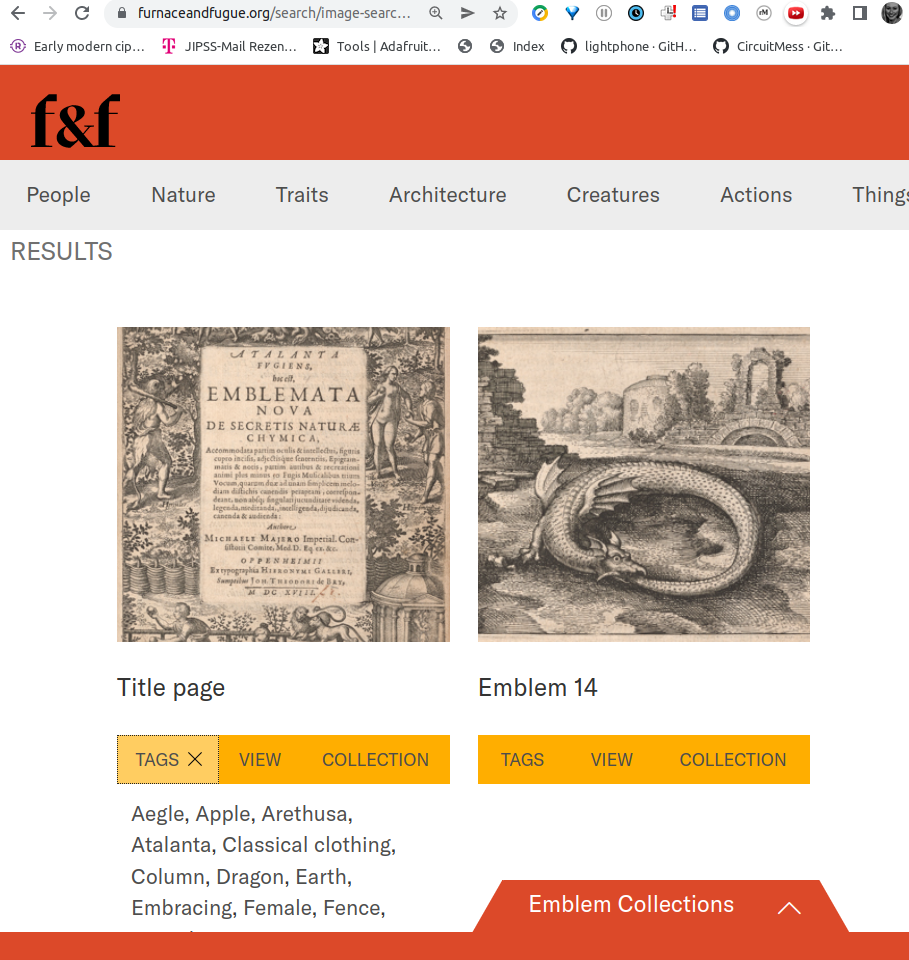
\includegraphics[width=\textwidth]{img/fnf2.png}
    \end{columns}
    
    
\end{frame}

%--------------------------------------------

\begin{frame}{From TEI to Edition}
What did all those examples have in common?
    \begin{itemize}\footnotesize
        \item all are digital editions
        \item all are based on data in TEI-XML
    \end{itemize}

That's what we want. -- How do we get there?

\metroset{block=fill}
\begin{block}{Remember}
\begin{itemize}\footnotesize
    \item XML is great for capturing \& long-term archiving data in its whole complexity
    \begin{itemize}
        \item[$\to$] \dots but also ends up chaotic with a lot of detail
        \item[$\to$] theoretically human-readable
        \item[$\to$] in practice, it's better to create a new representation of the data to read
    \end{itemize}
    \item \textbf{Desired result: }view/presentation, visualization and interaction with the data as a website (i.e. HTML data)
    \item \alert{$\to$ we need to transform the data}
\end{itemize}
\end{block}

\end{frame}

%--------------------------------------------


\begin{frame}{TEI Publication Tools}
There is a plethora of out-of-the-box solutions to make editions out of TEI data. 
$\to$
\alert{\href{https://wiki.tei-c.org/index.php/Category:Publishing_and_delivery_tools}{TEI List of Resources for Publishing and Delivery Tools}}, for example:
\begin{enumerate}
    \item teiPublisher
    \item EVT
    \item TEICHI
    \item Versioning Machine
    \item Boilerplate
    \item Oxgarage
    \item GAMS \dots 
\end{enumerate}

\end{frame}

%--------------------------------------------

\begin{frame}[allowframebreaks]{TEI Publisher: The Instant Publishing Toolbox}
    \begin{itemize}
        \item \protect\url{https://teipublisher.com/index.html}
        \item \protect\url{https://wiki.tei-c.org/index.php/TEI_Publisher}
        \item \protect\url{https://wiki.tei-c.org/index.php/TeiPublisher}
        \item \protect\url{http://hisoma.huma-num.fr/exist/apps/tei-publisher/index.html}
        \item ``Testimonial'': \href{https://digitalintellectuals.hypotheses.org/3912}{Florian Chiffoleau (2020), Blog Post: \emph{Publication of my digital edition -- Working with TEI Publisher.}}
    \end{itemize}
    
    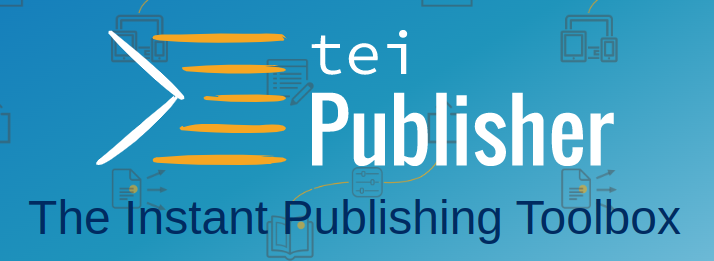
\includegraphics[width=0.7\textwidth]{img/tei-publisher1.png}
    
    \framebreak
    
    Demos:  \href{https://teipublisher.com/exist/apps/vangogh/let001.xml}{Van Gogh Letters} \sep \href{https://teipublisher.com/exist/apps/eebo/index.html}{Early English Books Online (EEBO)}
    
    \begin{columns}
    \column{0.33\textwidth}
    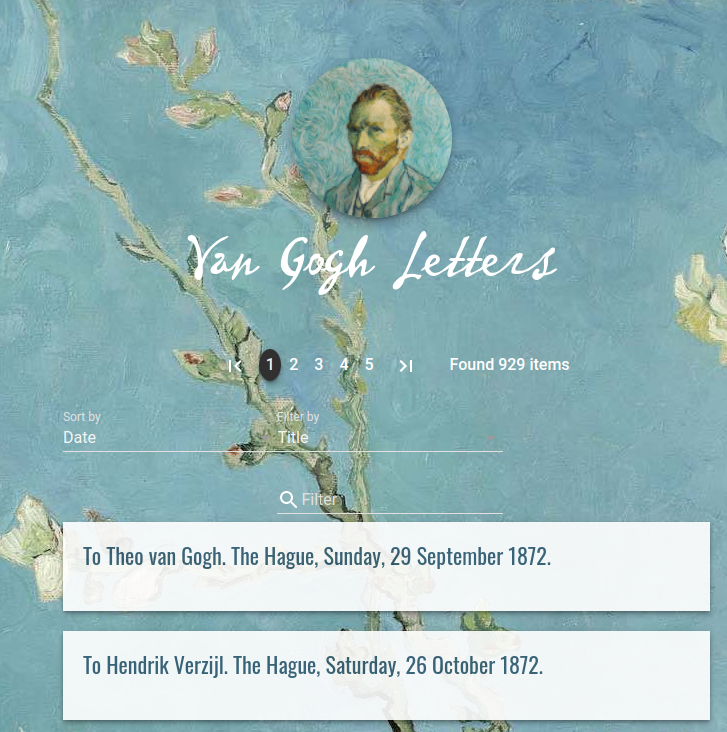
\includegraphics[width=\textwidth]{img/tei-publisher2.png}
    \column{0.33\textwidth}
    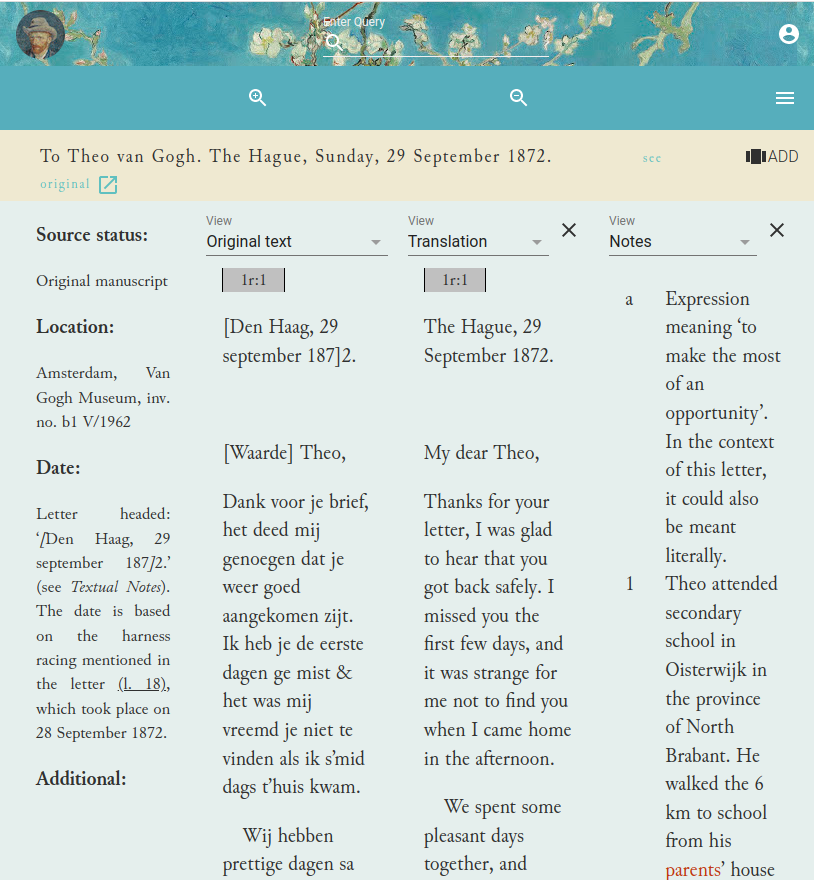
\includegraphics[width=\textwidth]{img/tei-publisher3.png}
    \column{0.33\textwidth}
    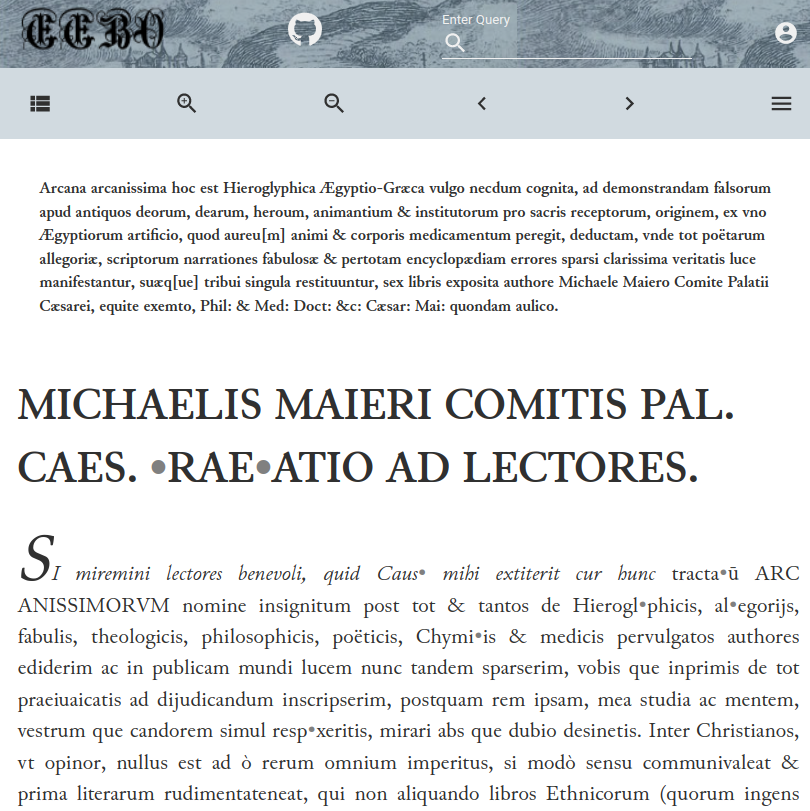
\includegraphics[width=\textwidth]{img/tei-publisher4.png}
    \end{columns}
\end{frame}


%--------------------------------------------

\begin{frame}{Edition Visualization Technology (EVT)}

\begin{columns}
\column{0.53\textwidth}
\begin{itemize}\scriptsize
    \item \protect\url{http://evt.labcd.unipi.it/} -- \protect\url{http://evt-project.sourceforge.net/}
    \item \protect\url{https://visualizationtechnology.wordpress.com/}
    \item Roberto Rosselli Del Turco, Giancarlo Buomprisco, Chiara Di Pietro, Julia Kenny, Raffaele Masotti and Jacopo Pugliese: \emph{Edition Visualization Technology: A Simple Tool to Visualize TEI-based Digital Editions}, Journal of the Text Encoding Initiative 8 (2014/15): Selected Papers from the 2013 TEI Conference “TEI Processing: Workflows and Tools”; \protect\url{https://doi.org/10.4000/jtei.1077}
    \item Del Turco, Roberto Rosselli. “Designing an Advanced Software Tool for Digital Scholarly Editions: The Inception and Development of EVT (Edition Visualization Technology).” \emph{Textual Cultures}, vol. 12, no. 2, 2019, pp. 91–111. JSTOR, \protect\url{www.jstor.org/stable/26821538}. 
\end{itemize}
\column{0.45\textwidth}
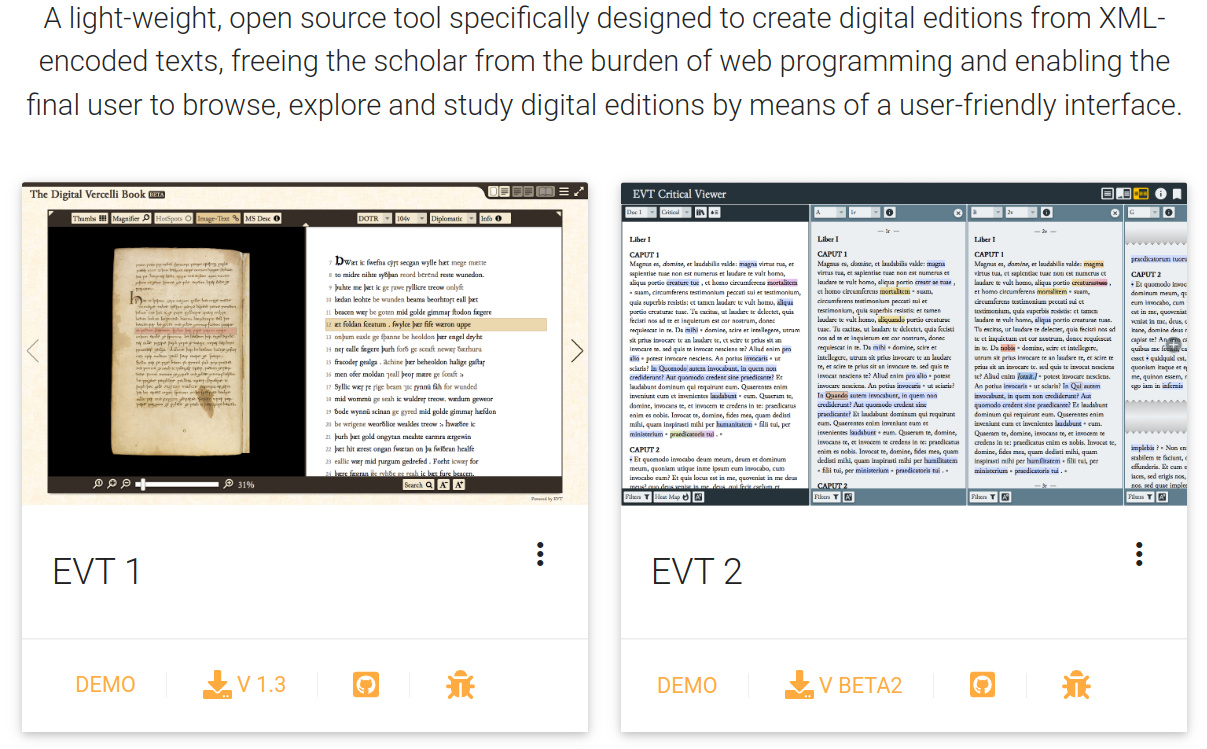
\includegraphics[width=\textwidth]{img/evt-example.png}
\end{columns}



\end{frame}

%--------------------------------------------

\begin{frame}{TeiCHI – Bringing TEI Lite to Drupal}


\begin{columns}
\column{0.38\textwidth}
\begin{itemize}\scriptsize
    \item TEIChi: a TEI lite integration into Drupal (\protect\url{http://teichi.org})
    \item Sebastian Pape, Christof Schöch and Lutz Wegner: \emph{TEICHI and the Tools Paradox. Developing a Publishing Framework for Digital Editions}, Journal of the Text Encoding Initiative 2 (2012): Selected Papers from the 2010 TEI Conference; \protect\url{https://doi.org/10.4000/jtei.432}
    \item \href{https://wiki.tei-c.org/index.php/TEICHI}{TEICHI wiki}
\end{itemize}
\column{0.68\textwidth}
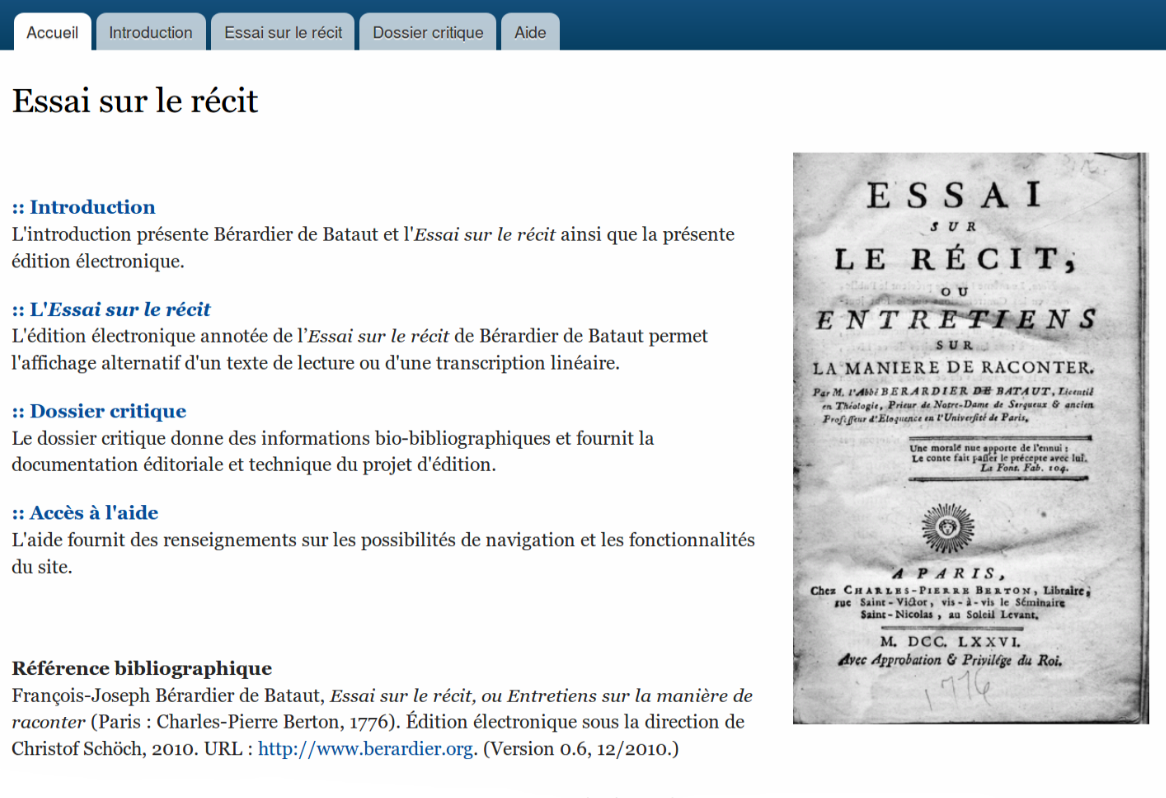
\includegraphics[width=\textwidth]{img/teichi-example.png}
\end{columns}



\end{frame}

%--------------------------------------------

\begin{frame}{The Versioning Machine}

\begin{itemize}\small
    \item Versioning Machine (\protect\url{http://v-machine.org/})
    \item \href{https://tei-c.org/activities/projects/the-versioning-machine}{The TEI Versioning Machine}
    \href{https://digitalhumanities.duke.edu/tools/versioning-machine}{Versioning Machine (Duke)}
\end{itemize}

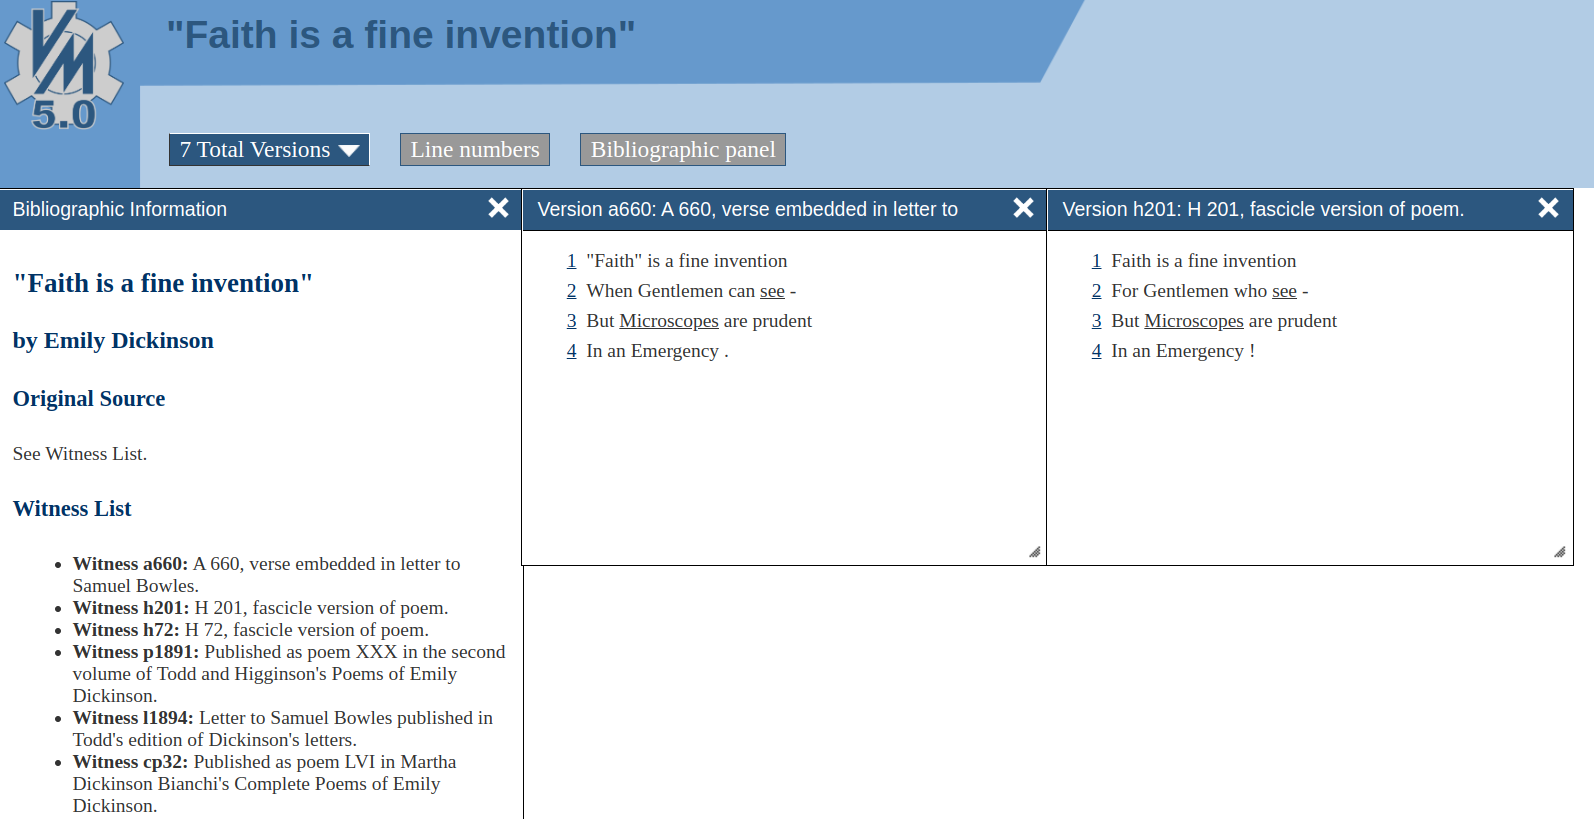
\includegraphics[width=0.9\textwidth]{img/tei-versioning-machine.png}

\end{frame}

%--------------------------------------------

\begin{frame}{TEI Boilerplate}

\begin{columns}
\column{0.48\textwidth}
\begin{itemize}\footnotesize
    \item \protect\url{http://teiboilerplate.org/}
    \item Boilerplate (\protect\url{http://dcl.slis.indiana.edu/teibp/})
    \item \href{http://dcl.slis.indiana.edu/teibp/content/demo.xml}{Demo}
    \item \href{https://wiki.tei-c.org/index.php/TEI_Boilerplate}{TEI Boilerplate Wiki}
    \item \href{https://www.i-d-e.de/wp-content/uploads/2014/07/boilerplate.pdf}{Slides on TEI Boilerplate}
    \item \href{http://tei.it.ox.ac.uk/Talks/2015-07-dhoxss/ex-boilerplate.pdf}{Exercise on TEI Boilerplate}
    \item \href{http://journalofdigitalhumanities.org/2-3/tei-boilerplate}{Poster on TEI Boilerplate}
\end{itemize}

\column{0.48\textwidth}
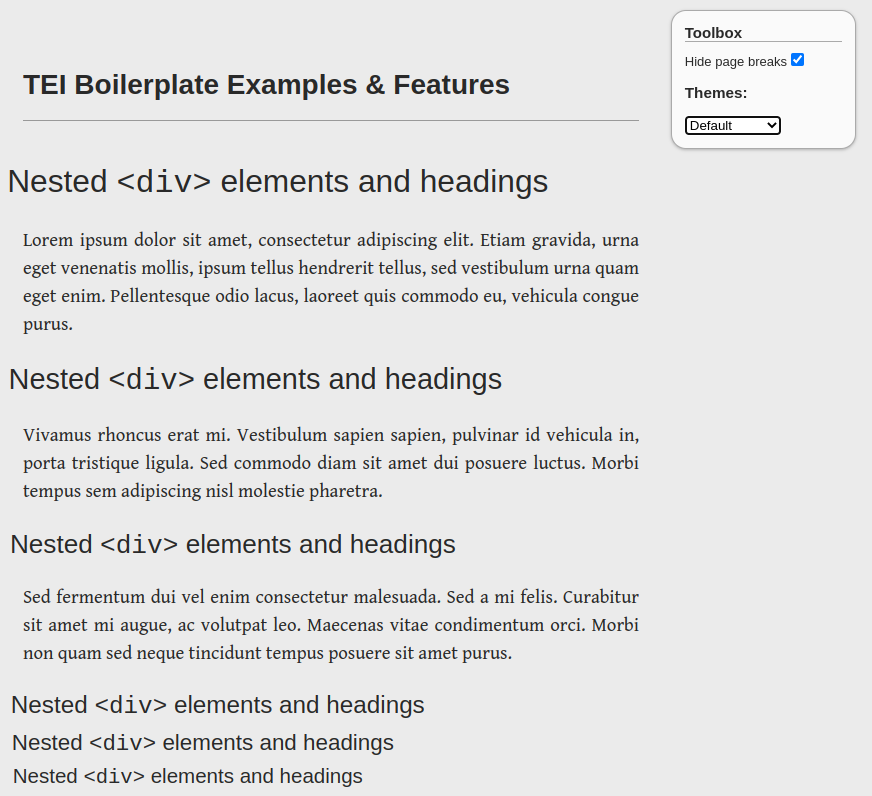
\includegraphics[width=\textwidth]{img/tei-boilerplate-example.png}
\end{columns}

\end{frame}

%--------------------------------------------

\begin{frame}{Oxgarage}
\metroset{block=fill}\footnotesize

\begin{columns}
\column{0.48\textwidth}
\begin{itemize}
    \item REST-based transformation web service for TEI documents (\protect\url{https://oxgarage.tei-c.org/})
    \item allows you to transform a number of (markup-based) formats to TEI or create them from TEI (\texttt{.html}, \texttt{.tex}, \texttt{.docx}, \dots)
    \item \href{https://tei-c.org/Vault/P5/3.6.0/doc/tei-xsl}{Based on TEI base stylesheets} (\protect\url{http://www.tei-c.org/Tools/Stylesheets/})
    \item[\textcolor{w3schools}{\faCheck}] very useful tool
    \item[\textcolor{alert}{\faClose}] not all TEI elements taken into account, not customizable
\end{itemize}
\column{0.48\textwidth}
\begin{block}{Oxgarage}
\dots offers a set of standard stylesheets to convert between TEI-encoded XML documents and other documents, mostly markup-based, such as \texttt{.docx}, \texttt{.html} or \texttt{.tex}. 

However, not all elements are covered and you have no control over how exactly they are processed. 
\end{block}
\end{columns}\medskip

Tools make things easier superficially but can come at a cost: potential bugs, less than ideal usability, lack of control and customizability:

\alert{$\to$ to customize we need to write our own transformation using XSL stylesheets}


\end{frame}



%--------------------------------------------

\begin{frame}[allowframebreaks]{GAMS (Humanities Asset Management System)}
\metroset{block=fill}
    \begin{columns}
    \column{0.44\textwidth}
    \begin{itemize}\small
        \item GAMS (\emph{Geisteswissenschaftliches Asset Management System} = AMS for the Humanities)
        \item based on \textbf{FEDORA} (\emph{Flexible Extensible Digital Object Repository Architecture}) = infrastructure dedicated to the persistent archival and management of resources considered to be worthy of long-term preservation.
    \end{itemize}
    \column{0.55\textwidth}
    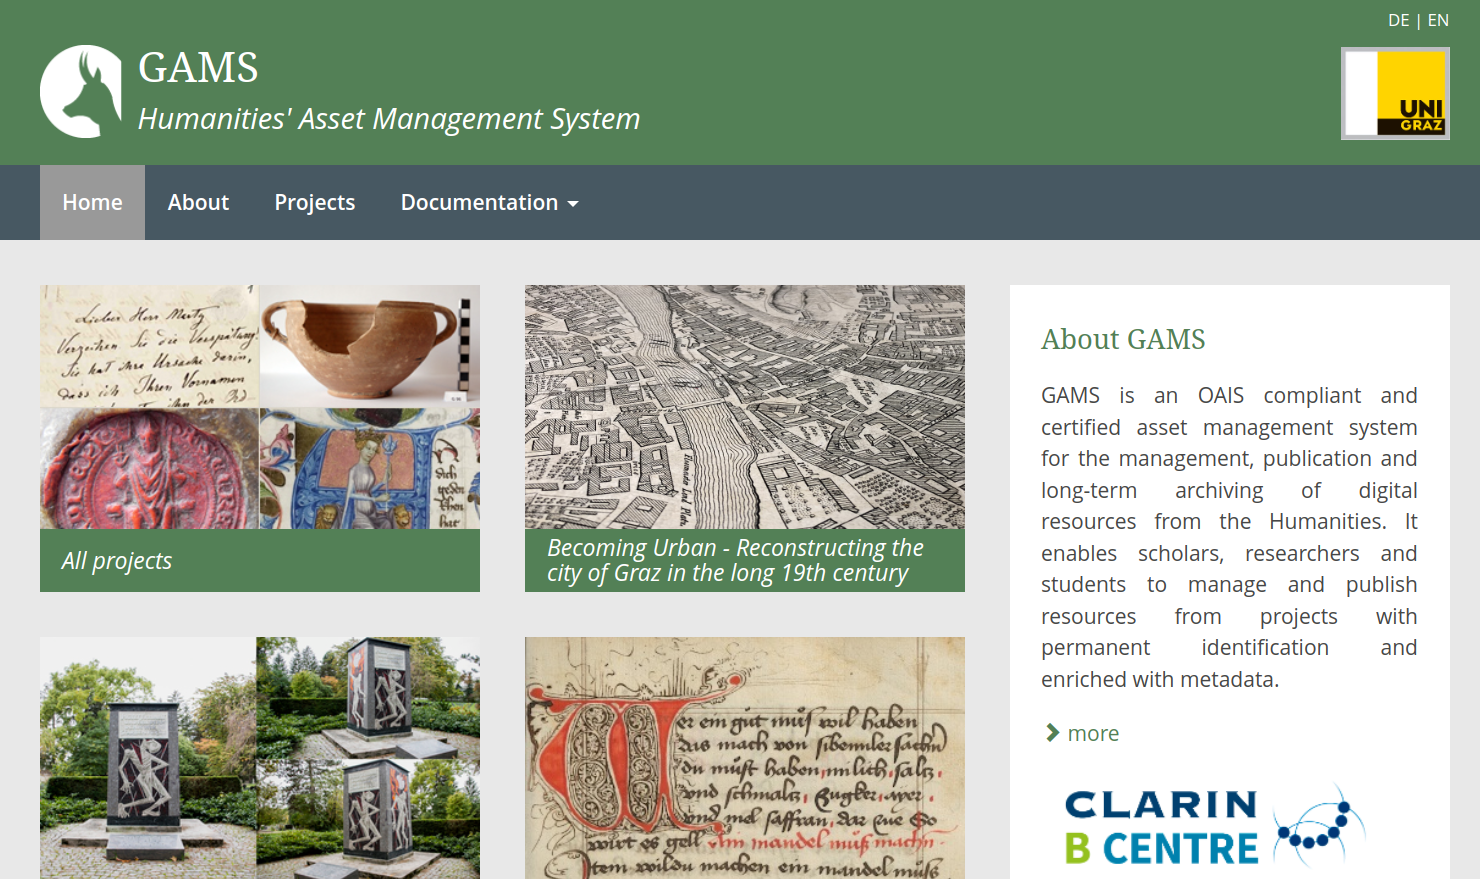
\includegraphics[width=\textwidth]{img/gams.png}
    \end{columns}
    \bigskip 
    
    \protect\url{https://gams.uni-graz.at}
    
    \framebreak
    
    \begin{columns}
    \column{0.58\textwidth}
    \begin{itemize}\small
        \item user access provided through the \textbf{Cirilo client}
        \item \textbf{functionalities:} object creation and management, versioning, normalization \& standards, choice of data formats.
        \item offers a plethora of \textbf{pre-defined content models} for data such as TEI, MEI, LIDO, SKOS, ontologies, R code and story lines
        \item $\to$ offers publication pipelines but is highly customizable
        \item more info: \protect\url{http://gams.uni-graz.at/doku}
    \end{itemize}
    \column{0.48\textwidth}
    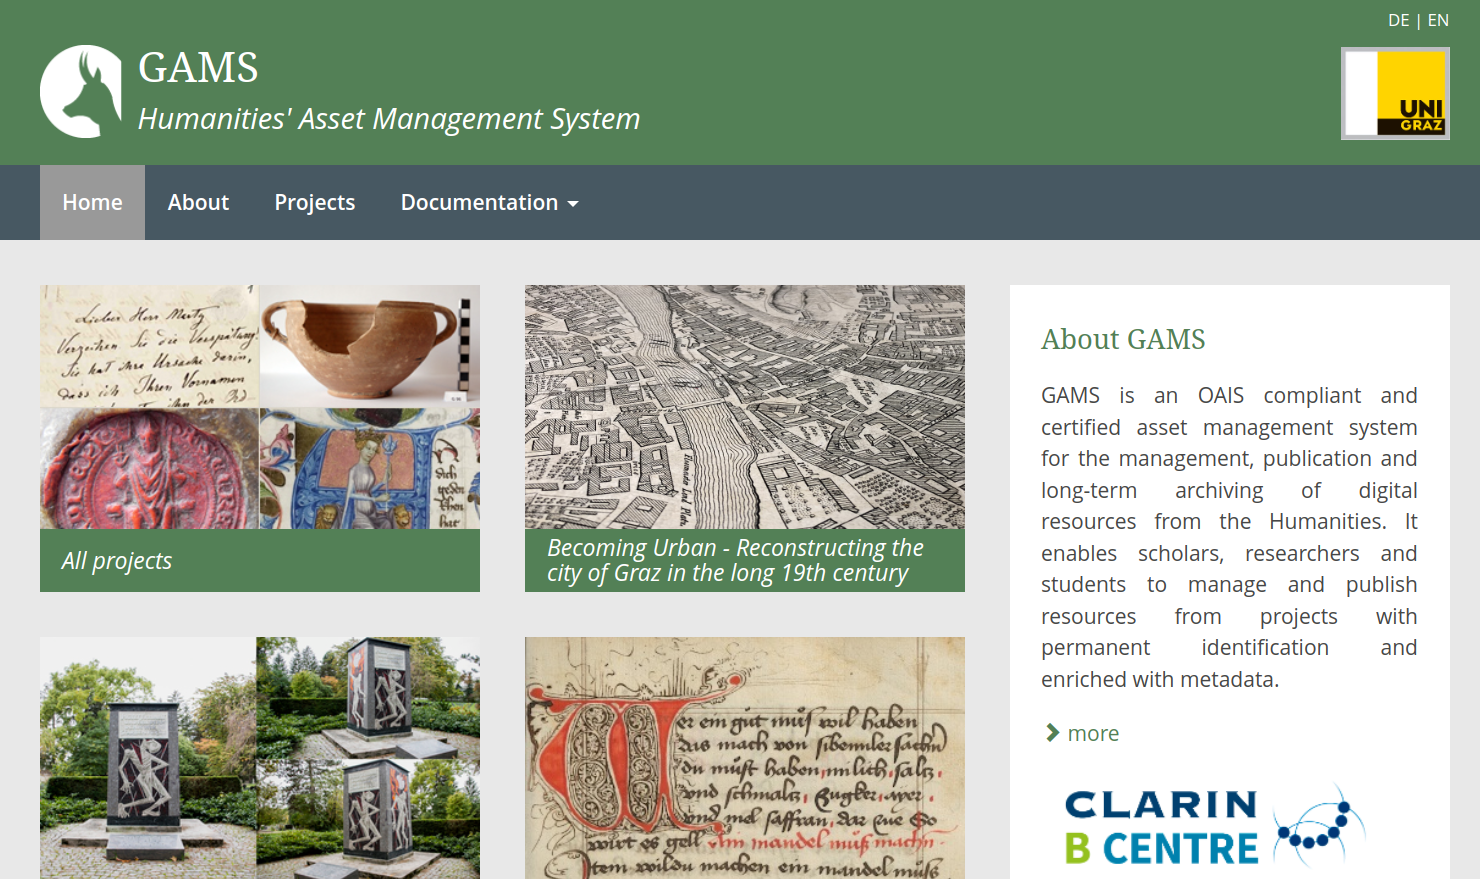
\includegraphics[width=\textwidth]{img/gams.png}
    \end{columns}
\end{frame}



%--------------------------------------------

\begin{frame}[allowframebreaks]{Long-term archiving heritage data}
\metroset{block=fill}
    \begin{columns}
    \column{0.4\textwidth}
    \begin{block}{Long-term preservation} denotes the process of maintaining, curating and keeping data usable over a long period of time (10+~years).
    \end{block}
    \column{0.58\textwidth}
    \begin{block}{Key functionalities of long-term archiving architectures include}
    \begin{itemize}\footnotesize
        \item persistent identification, 
        \item versioning, 
        \item support of different data formats, 
        \item management of associated metadata, 
        \item data export and retrieval, 
        \item security and scalability. 
    \end{itemize}
    
    Special emphasis is placed on 
    \begin{itemize}\footnotesize
        \item sustainability,
        \item citability \& 
        \item guarantee of long-term access to the contained resources. 
    \end{itemize}
    \end{block}
    \end{columns}
    
    \begin{block}{XML is great for long-term archiving!}
        Consequently, data formats and software used for preservation should follow \textbf{open source \& non-proprietary standards}; data is ideally encoded in an \textbf{unicode XML format}:
        \begin{itemize}
            \item plain text files are small
            \item human- \& machine-readable
            \item recognized standard stable since 1998
            \item more on XML later\dots
        \end{itemize}
    \end{block}
    
 \end{frame}



%--------------------------------------------

\begin{frame}[allowframebreaks]{Examples of data quality in GAMS}   
\metroset{block=fill}
    \begin{columns}
    \column{0.56\textwidth}
    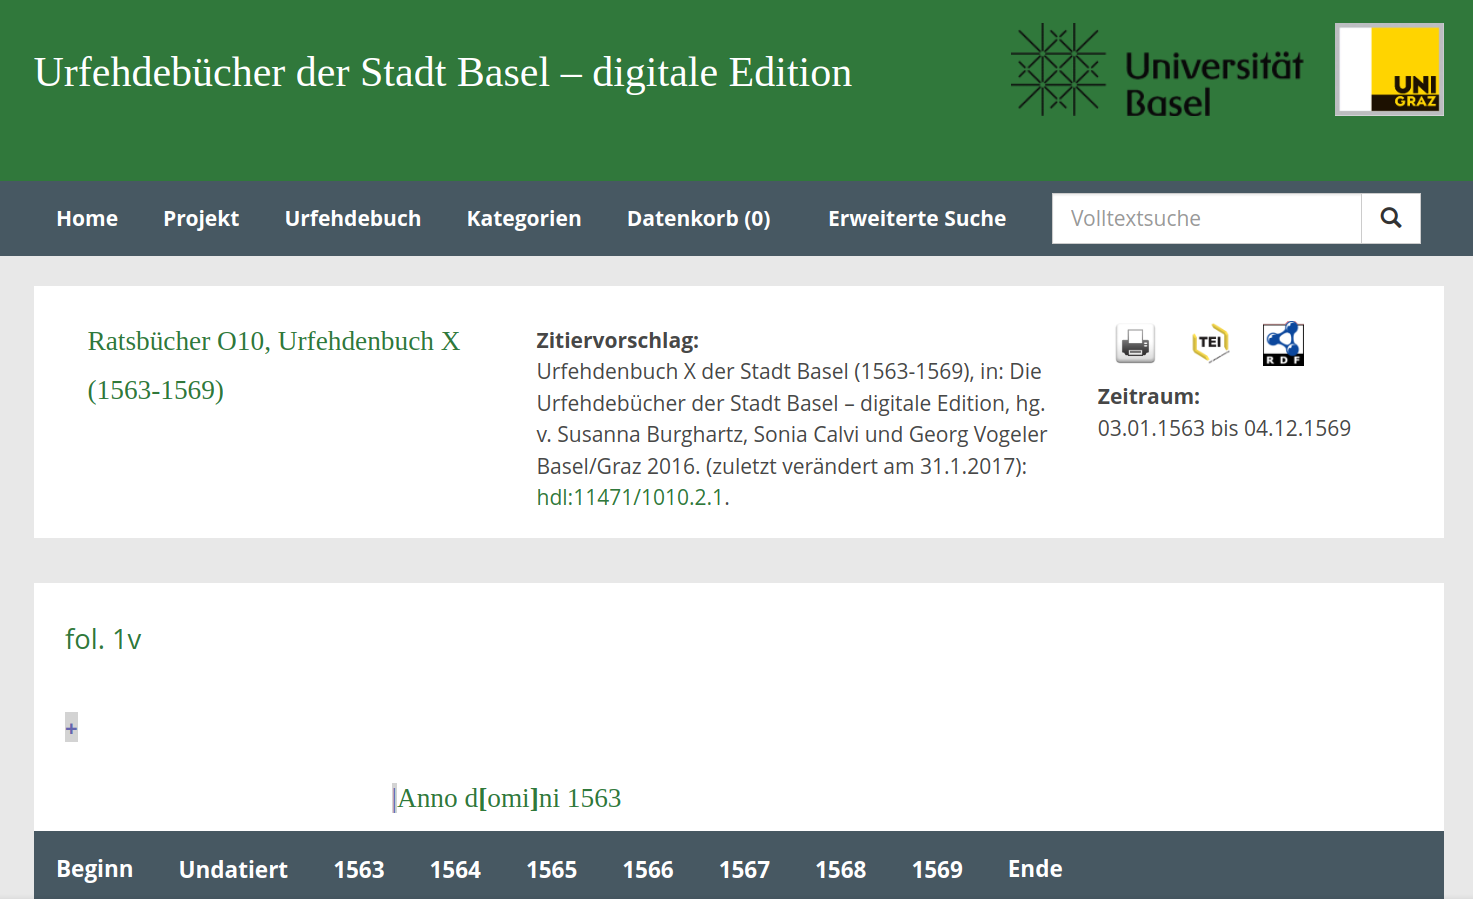
\includegraphics[width=\textwidth]{img/ufbas1.png}
    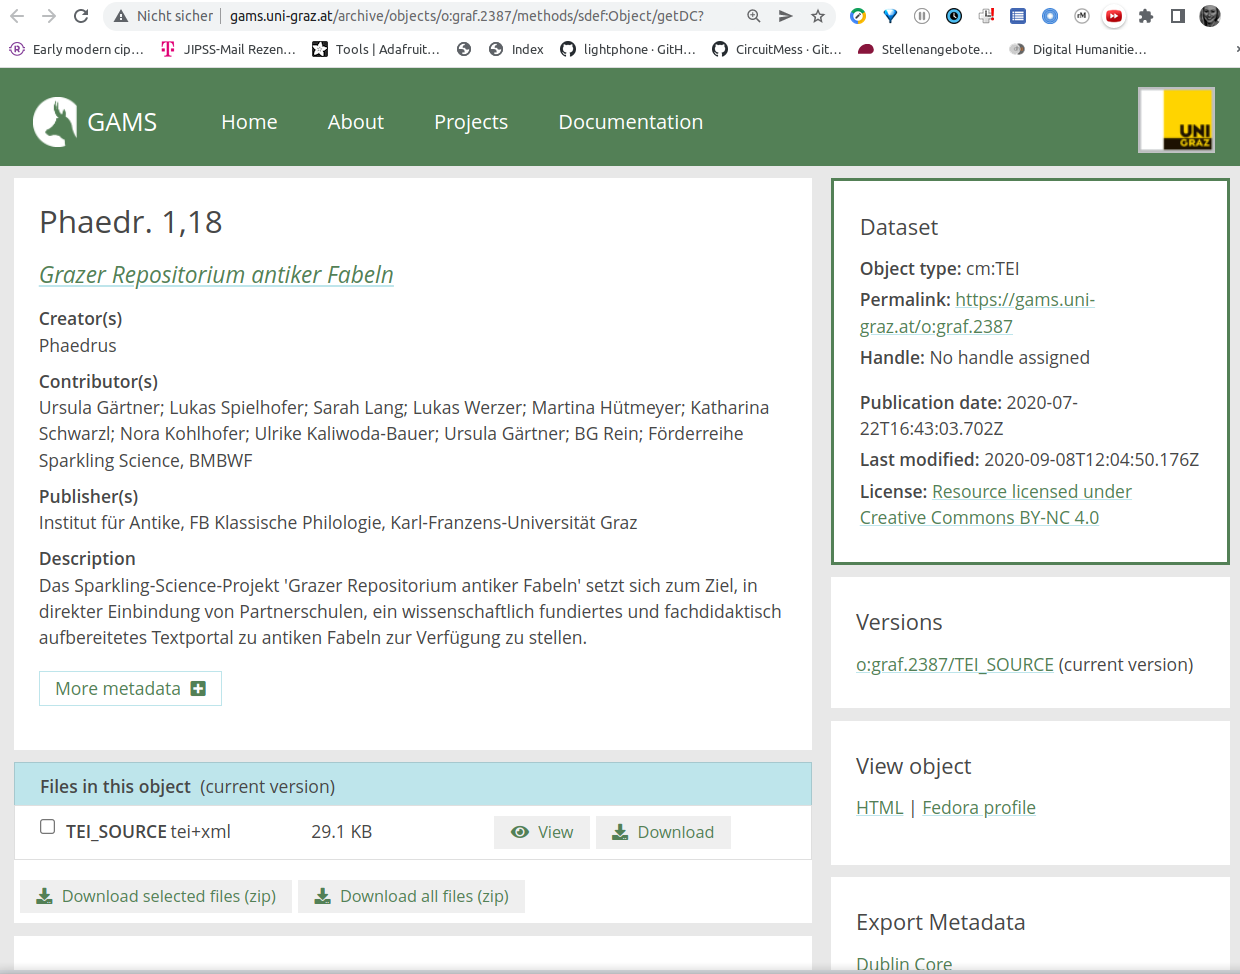
\includegraphics[width=\textwidth]{img/gams-graf-dc-metadata.png}
    \column{0.4\textwidth}
    \small
     $\leftarrow$ {\footnotesize \protect\url{http://gams.uni-graz.at/o:ufbas.1563}}
    \bigskip
    
    \begin{itemize}
        \item \textbf{top image:} info on recommended citation, downloadable source data in XML \& RDF
        \item \textbf{below:} `data view' of the Dublin Core (DC) metadata for an XML object in GAMS (ensuring citability, etc.)
    \end{itemize}
    \bigskip 
    
    $\leftarrow$ {\scriptsize \protect\url{http://gams.uni-graz.at/archive/objects/o:graf.2387/methods/sdef:Object/getDC?}}
    \end{columns}
    
    \begin{itemize}
        \item GAMS isn't an out-of-the-box tool -- it's something between a \textbf{Content Management System (CMS)}, a \textbf{repository} (long-term archiving) and a \textbf{publication platform}. 
        \item The XSLT transformations applied to files in GAMS are custom but there are \textbf{wippets} (standard javascript functionalities $\to$ \emph{widget + snippet}, \href{https://github.com/KONDE-AT/gams-wippets}{example here}) and \textbf{standard templates} which can be reused. 
        \item as a publication platform: presentation and long-term archiving, allowing for persistent access to the data, versioning, etc.
    \end{itemize}
    
    One more example: \protect\url{https://gams.uni-graz.at/beurb}
    \bigskip
    
    \begin{columns}
    \column{0.5\textwidth}
    
   \begin{block}{Metadata view on XML data}
    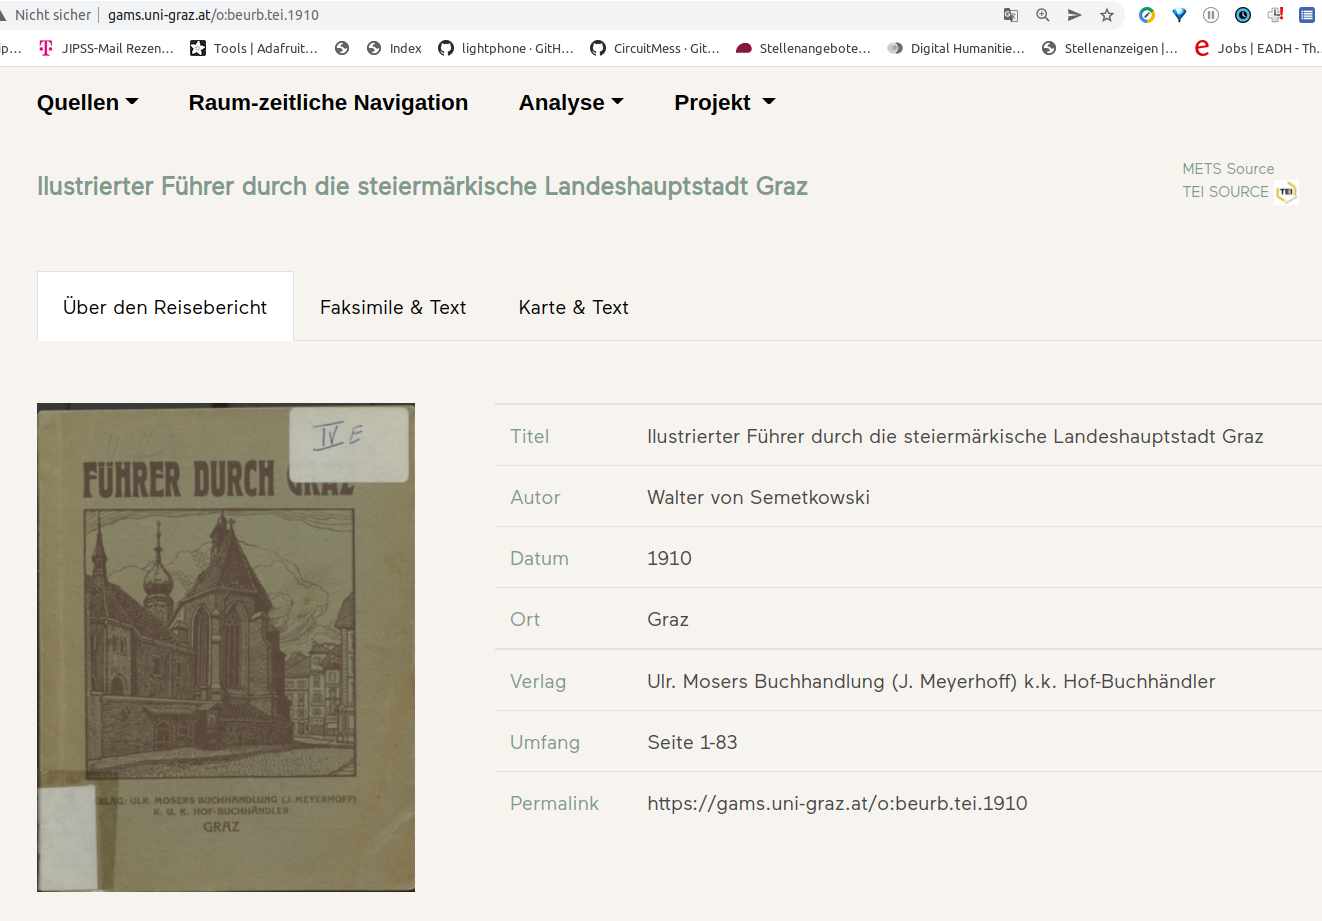
\includegraphics[width=\textwidth]{img/gams-beurb1.png}
   \end{block}
    \column{0.5\textwidth}
    \begin{block}{Map view linked to edited text} 
    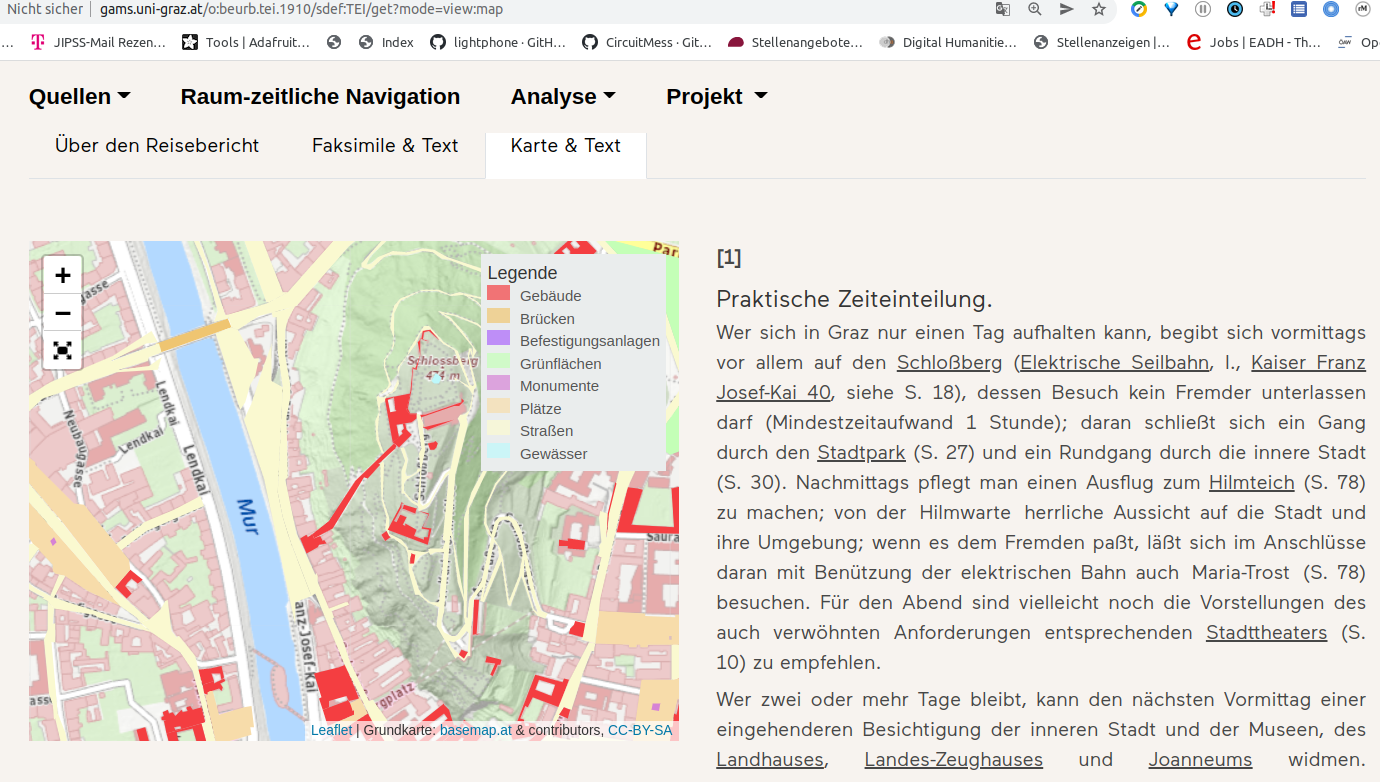
\includegraphics[width=\textwidth]{img/gams-beurb2.png}
    \end{block}
    \end{columns}
    Both views are created `on-the-fly' from the same XML file (=\emph{single source principle}, more on that later\dots).
\end{frame}


%-----------------------------------------------------



\begin{frame}[standout]

  \alert{Practice!}
  
  \normalsize
  Use \alert{\protect\url{https://oxgarage.tei-c.org/}} to transform some data to HTML. What do you notice? Do you like it or would you need to customize?
\end{frame}



